

%%%%%%%%%%%%%%%%%%%%%%%%%%%%%%%%%%%%%%%%%%%%%%%%%%%%%%%%%%%%%%%%%%%
%                                                                 %
%                           Background                            %
%                                                                 %
%%%%%%%%%%%%%%%%%%%%%%%%%%%%%%%%%%%%%%%%%%%%%%%%%%%%%%%%%%%%%%%%%%%


\chapter{Background} \label{c:background}

We will start by looking at some basic Probability Theory, and then move on to
Boolean Algebra. To conclude this section, we will introduce Block Ciphers and
the interesting properties surrounding them. We will only define concepts that
are needed as stepping stones to explaining Differential Cryptanalysis of Block
Ciphers, and thus exclude some fundamental theorems to certain sections that
are not needed. 

\section{Probability Theory}

What does it mean for an event to have a probability of occurring? You probably
have some intuitive understanding of what this means. For example, you will
probably be aware that when you flip a regular coin, you have a 50\% chance
that it will land with heads facing up, and a 50\% chance that it will land
with tails facing up. It is also easy to see that if you roll an unweighted
die, you have a 1 in 6 chance of landing on a particular number that was chosen
beforehand.

What if I ask you what the probability of you getting an even number on a die
is after you roll it? Most people would say there is a 50\% chance, since half
of the numbers are even and half of the numbers are odd. With this very
intuitive understanding of probability, we will define probability more
rigorously below.

Firstly, a \textbf{random experiment} is a procedure where the outcome cannot
be determined before the procedure is completed \cite[p.~57]{IntroStat}. In our
examples above, tossing a coin or rolling a die can be considered random
experiments.  The set of all possible outcomes to a random experiment is called
the \textbf{sample space} and a particular instance of conducting the random
experiment is known as a \textbf{trial}. An \textbf{event} in this context is a
subset of the sample space. So the coin landing with heads facing upwards, or
the die landing on a 3, or even the die landing on an even number would all be
examples of events occurring. However, an event that is a singleton in terms of
being a subset of the sample space is called an \textbf{elementary event} .
Thus, only getting heads on a coin toss, or getting a 3 on a die roll can be
considered elementary events. Finally we will end off with a definition about
how events relate to each other.

\begin{defn}
For $S$, some sample space, let $A, B \subset S$ be events. Then they are
called \textbf{mutually exclusive} if $A \cap B = \emptyset$.
\end{defn}

So what is probability then? Kolmogorov, often considered the father of
probability, defined it as follows: 

\begin{defn}
Suppose $S$ is a sample space for a random experiment. Then, for all events $A
\subset S$, we define the \textbf{probability} of $A$, denoted $Pr(A)$, to be a
real number with the following properties:
\begin{enumerate}
\item $0 \leq Pr(A) \leq 1$
\item $Pr(S) = 1$ and $Pr(\emptyset) = 0$, where $\emptyset$ is the empty set or \textbf{null event}.
\item For $A, B \subset S$, if $A \cap B = \emptyset$ then $Pr(A \cup B) = Pr(A) + Pr(B)$
\end{enumerate}
\end{defn}

Now that we have made precise the definition of probability, we can look
into calculating probabilities of events occurring. Eventually we will
use this to show how we can calculate the probability of a set of 
independent events. But first, a few theorems:

\begin{thm}
If $A_1, A_2, ... ,A_n$ are pairwise mutually
exclusive (in other words, for $i \neq j, A_i \cap A_j = \emptyset$), then
\begin{equation}
    Pr(A_1 \cup A_2 \cup ... \cup A_n) = \
    Pr(A_1) + Pr(A_2) + ... + Pr(A_n)
\end{equation}
This can be written concisely as
\begin{equation}
    Pr\left(\bigcup _{i=1}^nA_i\right) = \sum _{i=1}^nPr(A_i) 
\end{equation}
\end{thm}

\begin{prf}
This proof can be obtained by the repeated use of Axiom 3.

We know that for any $A_i, A_j \in \{A_1, A_2, ... , A_n\}$,
$A_i$ and $A_j$ are mutually exclusive.
Thus, by use of Axiom 3, we have 
\begin{equation} \label{e:pr1}
Pr\left(\bigcup _{i=1} ^n A_i\right) = Pr\left(\bigcup _{i=1} ^{n-1} A_i\right) + Pr(A_n)
\end{equation}
But it can also be noted that 
\begin{equation}
Pr\left(\bigcup _{i=1} ^{n-1} A_i\right) = Pr\left(\bigcup _{i=1} ^{n-2} A_i\right) + Pr(A_{n-1})
\end{equation}
Substituting into \ref{e:pr1}, we get
\begin{equation}
Pr\left(\bigcup _{i=1} ^n A_i\right) = Pr\left(\bigcup _{i=1} ^{n-2} A_i\right) + Pr(A_{n-1}) + Pr(A_n)
\end{equation}
Repeating this process, it is easy to see that
\begin{equation} 
Pr\left(\bigcup _{i=1} ^n A_i\right) = Pr(A_{1}) + ... + Pr(A_{n-1}) + Pr(A_n)
\end{equation}
The result follows. \qed
\end{prf}

Recalling that elementary events are mutually exclusive, if we know the
probability of each elementary event, we can calculate the probability of any
event by summing the probabilities of the elementary events it contains. This
however can be tedious, so we look for a better way of calculating
probabilities of a certain class of problems. They are the class of problems
where by elementary events are equiprobable, that is having an equal
probability of occurring. Thus, if there are $N$ elementary events in our
sample space, each elementary event should have a probability of $\frac{1}{N}$
of occurring. Thus, to calculate the probability of an arbitrary event $A$
occurring, we could sum $\frac{1}{N}$ $n(A)$ times, where $n(A)$ denotes the
number of elementary events contained in $A$, since $A$ is just the union of
elementary events contained in $A$. It is easy to see then that
\begin{equation}
Pr(A) = \frac{1}{N} \times n(A)
\end{equation}

Now that we have a fast way of computing probabilites of arbitrary events
for which we know the probability of elementary events, we can consider
events that are independant of one another.

\begin{defn}
Let $A$ and $B$ be two events in a sample space $S$. Then the 
\textbf{conditional probability} of the event B given that the event A has
occurred, denoted by $Pr(B|A)$, is
\begin{equation}
Pr(B|A) = \frac{Pr(A \cap B)}{Pr(A)}
\end{equation}
\end{defn}

What follows directly from the definition of conditional probability, is 
what it means for events to be independent.

\begin{defn}
Events are called \textbf{independent} if the outcome of one event does
not affect the outcome of another. That is, for $A, B \subset S$
\begin{equation}
Pr(B|A) = Pr(B).
\end{equation}
\end{defn}

What however happens when we want to find the probability of two independent
events both occurring? The next theorem tells us.

\begin{thm}\label{t:indep}
Let $A, B \subset S$ be two independent events. Then the probability of 
both $A$ and $B$ occurring, $Pr(A \cap B)$, is given by
\begin{equation}
Pr(A \cap B) = Pr(A) \times Pr(B).
\end{equation}
\end{thm}

\begin{prf}
$A$ and $B$ are independent, thus 
\begin{align*}
Pr(B|A) &= Pr(B)\\
\frac{Pr(A \cap B)}{Pr(A)} &= Pr(B)\\
Pr(A \cap B) &= Pr(A) \times Pr(B)\hfill\qed\\
\end{align*}
\end{prf}

However, for Block Ciphers we are interested in the probability of 
multiple independent events occurring together. Thus, we finish
off this section of probability theory by proving the following
very useful theorem.

\begin{thm}
Let $A_1, ... , A_n$ be independent events, then 
\begin{equation}
Pr\left(\bigcap _{i=1} ^n A_i \right) = Pr(A_1) \times ... \times Pr(A_n)
\end{equation}
\end{thm}

\begin{prf}
We prove this inductively by first examining the case of $n = 2$.
We know
\begin{equation}
Pr\left(\bigcap _{i=1} ^2 A_i \right) = Pr(A_1) \times Pr(A_2)
\end{equation}
from Theorem \ref{t:indep}
Now we examine the case where $n = m$ for some arbitrary $m \in \N$. 
Since $A_1, ... , A_m$ are independent events, it is easy to see that
$\bigcap _{i=1} ^{m-1} A_i$ and $A_m$ are independent events. Thus we
can see that
\begin{equation}
Pr\left(\bigcap _{i=1} ^m A_i \right) = Pr\left(\bigcap _{i=1} ^{m-1} A_i \right) \times Pr(A_m)
\end{equation}
holds. However,
\begin{equation}
Pr\left(\bigcap _{i=1} ^m A_i \right) \times Pr(A_{m+1}) = Pr\left(\bigcap _{i=1} ^{m-1} A_i \right) \times Pr(A_m) \times Pr(A_{m+1})
\end{equation}
yields
\begin{equation}
Pr\left(\bigcap _{i=1} ^{m+1} A_i \right) = Pr\left(\bigcap _{i=1} ^{m} A_i \right) \times Pr(A_{m+1}).
\end{equation}
Expanding out, we get
\begin{equation}
Pr\left(\bigcap _{i=1} ^{m} A_i \right) = (...(Pr(A_1) \times Pr(A_2)) \times Pr(A_3)) \times ... Pr(A_m).
\end{equation}
and the result follows by induction for every $n \in \N$.
\end{prf}

\section{Boolean Algebra}
In order to understand how many Block Ciphers work, we will have to take a 
look at Boolean Algebra, that is, the logical calculus of truth values.
In particular we will look at the operation known as the `exclusive or', 
commonly known as XOR and represented by the symbol `$\oplus$'.

\subsection{XOR}
\begin{defn}
The XOR of two boolean values is true if either one of the values is true,
and is false if both are true, or both are false.
\end{defn}
In simpler terms, we can view it as a function that takes two inputs, and 
returns true if either the one value or the other is true, but not both.
As we are dealing with True and False values, we will use the more compact
notation of representing $True$ as $1$, and $False$ as $0$. 

Thus, the truth table for the XOR operation is given as follows:
\begin{center}
\begin{tabular}{|r|r|r|}
\hline
$A$ & $B$ & $A \oplus B$ \\\hline
0 & 0 & 0 \\\hline
0 & 1 & 1 \\\hline
1 & 0 & 1 \\\hline
1 & 1 & 0 \\\hline
\end{tabular}
\end{center}

This can be compactly noted in the operation table below:
\begin{center}
\begin{tabular}{|r|r|r|}
\hline  
& 0 & 1 \\\hline
0 & 0 & 1 \\\hline
1 & 1 & 0 \\\hline
\end{tabular}
\end{center}

What the above table is saying, is that $0 \oplus 0 = 1 \oplus 1 = 0$.
Likewise, $0 \oplus 1 = 1 \oplus 0 = 1$.

\begin{rem}
It is easy to see that this operation is equivalent to addition in $\F_2$,
that is, the finite field of order 2.
\end{rem}

\subsection{Boolean Vectors}
We can examine collections of truth values in a particular order as an
$n$-vector of boolean values. 

This results in us being able to define XOR on these vectors:

\begin{defn}
Let $A = (a_1, a_2, ... , a_n), B = (b_1, b_2, ... , b_n) \subset \{0,1\}^n$ be two Boolean $n$-vectors. Then,
\begin{equation}
A \oplus' B = (a_1 \oplus b_1, a_2 \oplus b_2, ... , a_n \oplus b_n)
\end{equation}
where $\oplus'$ represents the component-wise XOR of boolean vectors.
\end{defn}

\begin{rem}
Since it will never be ambiguous as to whether we are XORing boolean
values or boolean vectors, we will drop the use of $\oplus'$ and just
use $\oplus$ to denote XOR of both values and vectors.
\end{rem}

\subsection{Bits}
We have already seen how it is convenient to represent truth values as 1s
and 0s in the previous subsection. We will now look at the primary way of
compactly representing Boolean vectors - namely that of bit strings.

Firstly, let's take a look at some Computer Science terminology:
\begin{itemize}
\item A \textbf{bit} or binary digit is variable which holds either a $0$ or a $1$.
\item A \textbf{bit string} is a sequence of 1 or more bits.
\end{itemize}

We can see that the definition of a bit fits well with our representation of
boolean values in the previous section. In fact, in the space of Boolean
Algebra, the term bit is actually used to denote truth values given by this 
numerical representation.

Thus, if we consider a Boolean $n$-vector $(a_1, a_2, ..., a_n)$, we
can represent this as a bit string of length $n$, of the form $a_1a_2...a_n$.
Furthermore, our definition of XOR applies to bits as well and a bit string can
be bit-wise XOR'd with a string of the same length, by taking the
component-wise XOR of the corresponding Boolean vector. This results in the
following definition of a bit-wise XOR:

\begin{defn}
Let $A = a_1a_2...a_n$ and $B = b_1b_2...b_n$ be two bit strings of length $n$. 
Then $A \oplus B$ is defined to be the bit string representation of 
$A' \oplus B'$ where $A' = (a_1, a_2, ..., a_n), B' = (b_1, b_2, ..., b_n) \subset \{0,1\}^n$,
the Boolean vector representation of $A$ and $B$.

\end{defn}

\begin{example}
Suppose we wanted to XOR 101011 with 011010. We could convert the bit strings
into their boolean tuple representation and component-wise XOR them. 

Thus, 
\begin{align*}
101011 \oplus 011010 
                     &= (1, 0, 1, 0, 1, 1) \oplus (0, 1, 1, 0, 1, 0)\\ 
                     &= (1 \oplus 0, 0 \oplus 1, 1 \oplus 1, 0 \oplus 0, 1 \oplus 1, 1 \oplus 0)\\
                     %&= (1 \oplus 0) + (0 \oplus 1) + (1 \oplus 1) + (0 \oplus 0) + (1 \oplus 1) + (1 \oplus 0)\\
                     %&= (1) + (1) + (0) + (0) + (0) + (1)\\
                     &= (1, 1, 0, 0, 0, 1)\\
                     &= 110001
\end{align*}
\end{example}

You might notice that this operation can be described as taking the first bit
string, and flipping a bit wherever you see a 1 as the corresponding bit in
the second bit string.

\begin{rem}
Often, for the sake of brevity, we will use the decimal or hexadecimal 
representation of a number rather than it's binary representation. The reader
is assumed to have knowledge of number systems and converting between
variously based number systems.
\end{rem}

\section{Block Ciphers}
We will be considering an attack on Block Ciphers later, and thus it makes sense
to introduce Block Ciphers as part of the background.  In short, Block Ciphers
can be defined as algorithms that operate on a fixed number of bits, using some
sort of symmetric key. \cite[]{handbook} 

Alright, let's take a step back and try understand what that means. Given some
plaintext, a block cipher will convert fixed-size blocks of that plaintext into
the same size blocks of ciphertext during the encryption stage. The way in which
it does this depends on the type of block cipher in discussion, but usually this
involves XORing in a secret key in some way. Furthermore, since this key is
symmetric, it can be used with the same block cipher to reverse the process, and
convert ciphertext that has been generated by this particular block cipher, back
into plaintext.

In particular, a block cipher is a combination of two paired algorithms, E for
encryption, and D for decryption. Both algorithms accept two inputs, an input box
of size $n$ bits, and a key of size $k$ bits and both yield an $n$-bit output block. 

How could we make this definition more precise though? With our intutive
understanding of a Block Cipher, we can define it mathematically as follows:

\begin{defn}
If $K$ is an input key of bit length $k$, and $P$ is a string of input bits
of length $n$, let us consider a function 
\begin{equation} \label{block-encrypt}
E_K(P) := E(K,P): \{0,1\}^k \times \{0,1\}^n \rightarrow \{0,1\}^n
\end{equation}

For each $K$ and output of $E_K(P) = C$, the function $E_K(P)$ is required to be an invertible mapping
on $\{0,1\}^n$, with the inverse defined as:
\begin{equation}\label{block-decrypt}
E_K ^{-1}(C) := D(K,C): \{0,1\}^k \times \{0,1\}^n \rightarrow \{0,1\}^n
\end{equation}
such that
\begin{equation}
\forall K\ D_K(E_K(P)) = P
\end{equation}
holds.

Then the pair $(E_K, D_K = E_K ^{-1})$ constitutes a block cipher. 
\end{defn}

\begin{rem}
In the above:
\begin{itemize}
\item $k$ is known as the \textbf{key size}
\item $n$ is known as the \textbf{block size}
\item $C$ is known as the \textbf{ciphertext}
\item $P$ is known as the \textbf{plaintext}
\end{itemize}
\end{rem}

There are different types of block ciphers, but for the purposes of this paper,
we will focus on a specific type of iterated block cipher, known as a
Substitution-Permutation Network (SPN). There are other types of block ciphers,
such as Feistel ciphers, but these are beyond the scope of our discussion.
What makes SPNs different from other block cipher implementations, is the way 
the symmetric key is mixed in with the plaintext to form ciphertext. 

Iterated block ciphers are block ciphers in which the secret key used to
generate the various subkeys or ``round keys'' that are mixed in over multiple
rounds. At each round, a ``round function'' takes the previous round's output
as input, with the first round using the plaintext as input. Thus, these round
functions are chained together to form our iterated block cipher. In the case
of an SPN, the round function is made up of a Key-mixing stage, a Substitution box (S-box)
and a Permuation box (P-box), in that order.

Looking at figure \ref{fig:SP}, we can see this in action. In the next subsections
we will discuss what S-boxes and P-boxes are.
\begin{figure}
\begin{center}
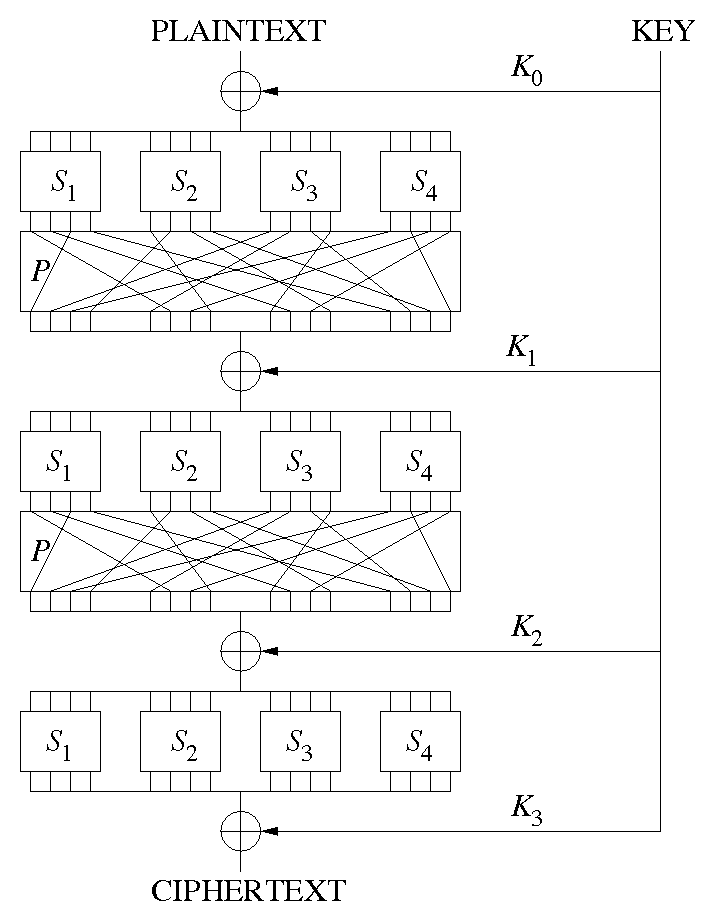
\includegraphics[scale=0.50]{spn.png} 
\caption{Substitution-Permutation Network \cite[]{gabore}}
\label{fig:SP}
\end{center}
\end{figure}

\subsection{Vectorial Boolean Functions (S-boxes)}
A large part of understanding Block Ciphers, and how to attack them, will be
tied up in understanding S-boxes (which are types of Vectorial Boolean
Functions). This section will deal with introducing and explaining them, along
with a few examples.

\begin{defn}
Any bijection $S:\{0,1\}^n \rightarrow \{0,1\}^m$ which maps boolean
$n$-vectors to boolean $m$-vectors, is called a \textbf{Substitution-box}
(S-box). Where $n = m$ we call $n$ the block size, and we refer to an S-box
with block size $n$, as an $n$-bit S-box. In the case that $n \neq m$,
we will refer to such an S-box as an $(n \times m)$-bit S-box.
\end{defn}

\begin{rem}
For the sake of convenience, we will continue to discuss Block-Ciphers
in terms of $n$-bit S-boxes, unless otherwise stated.
\end{rem}

What immediately follows from the fact that S is a bijection, is that
the inverse $S^{-1}$ exists, and that we can reverse the S-box.

\begin{example}
A very simple, but not very useful, S-box would be one operating on $n$-vectors, which just maps
every element to itself (the so called identity S-box).
\begin{equation}
S_{id}: \{0,1\}^n \rightarrow \{0,1\}^n
\end{equation}
where
\begin{equation}
S_{id}(x) = x
\end{equation}

\end{example}

\begin{example}
Let's consider a simple 3 bit S-box. Since there are only 3 bits, we have 
$2^3 = 8$ possible inputs. Since S-boxes are bijections, we can only have
8 possible outputs. Thus, we can think of an S-box as a type of look-up
table.

\begin{center}
\begin{tabular}{|r|r|}
\hline
$x$ & $y = S(x)$ \\\hline
$000$ & $010$ \\\hline
$001$ & $110$ \\\hline
$010$ & $000$ \\\hline
$011$ & $100$ \\\hline
$100$ & $011$ \\\hline
$101$ & $001$ \\\hline
$110$ & $111$ \\\hline
$111$ & $101$ \\\hline
\end{tabular}
\end{center}

We can however reverse the S-box, taking $x$ to be the subject of our formula.
So instead of $y = S(x)$, we get $x = S^{-1}(y)$. Looking at the previous
table like this, we get:

\begin{center}
\begin{tabular}{|r|r|}
\hline
$y$ & $x = S^{-1}(y)$ \\\hline
$000$ & $010$ \\\hline
$001$ & $101$ \\\hline
$010$ & $000$ \\\hline
$011$ & $100$ \\\hline
$100$ & $011$ \\\hline
$101$ & $111$ \\\hline
$110$ & $000$ \\\hline
$111$ & $110$ \\\hline
\end{tabular}
\end{center}

\end{example}


\subsection{P-boxes}
From the previous section, we can see here is that S-boxes serve to obscure the
relationship between plaintext and ciphertext, thereby providing good
\textbf{confusion} for the Block Cipher as defined by \cite{shannon}. Another
property that we want for a good Block Cipher would be that small changes in
our plaintext will result in completely different ciphertext. More formally, we
want that redundancy, or non-message bits, in the statistics of our plaintext
be dissipated in the statitics of our ciphertext, known as Shannon's property
of \textbf{diffusion}. To achieve that, we use something called a Permutation-box.

\begin{defn}
A \textbf{Permutation-box} or P-box is a method of bit-shuffling used to permute
or transpose bits across bit strings.
\end{defn}

Since a P-box permutes bits over bit strings, we can put a P-box immediately
after an S-box to send output bits from one S-box to a different input location
for the next round. We refer to such an S-box followed immediately by a P-box
as an SP-box.
